\cotefile{35}
\scanpage{2}
\noindent\hfill\margin{\handwritten{\unsure{zurück} \unsure{an|au} G.}}\par

\noindent SGA 7\qquad Groupe de Monodromie en Géométrie Algébrique

\reversemarginpar
\noindent\margin{\handwritten{\unsure{Gr|Gro}}}I\quad G\deleted{\unsure{ad|ed}}énéralités sur le g\deleted{\unsure{o}}roupe de monodromie locale. Le théorème de monodromie par voie arithmétique.

\noindent\margin{\handwritten{Gr}}II\quad Cas d'action\deleted{s} résoluble\deleted{s} d'ungroupe fondamental (variante du \deleted{groupe} théorème de monodromie).

\noindent\margin{\handwritten{Gr}}III\quad Le théorème de monodromie par voie géométrique.\normalmarginpar
\margin{\handwritten{\figure{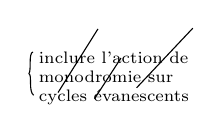
\begin{tikzpicture}[x=1cm,y=1cm,scale=.86,transform shape]
\node[anchor=north west,align=left,inner sep=0pt,font=\scriptsize] at (.14,.06)
{\deleted{\unsure{inclure} l'action \unsure{de}}\\
 \deleted{\unsure{monodromie} sur}\\
 \deleted{\unsure{cycles} évanescents}};
\draw (.06,.05) .. controls (-.01,.03) and (.04,-.22) .. (0,-.27)
 .. controls (.05,-.29) and (-.01,-.53) .. (.07,-.59);
\draw (.43,-.55)--(1.02,.39) (.97,-.64)--(1.36,-.04) (1.59,-.48)--(2.42,.40);
\end{tikzpicture}}}}

\reversemarginpar
\noindent\margin{\handwritten{Gr}}IV\quad Propriétés générales des groupes de cycles évanescents. Cas des points singul\deleted{\unsure{ei|ee}}iers isolés de la fibre spéciale.

% slanted
\noindent\margin{\handwritten{Gr\par
\figure{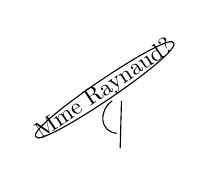
\begin{tikzpicture}[scale=.84,transform shape]
\begin{scope}[rotate=34,transform shape]
\node[inner sep=1.1pt] (q) {Mme Raynaud?};
\draw (q.west) .. controls (q.north west) and ([xshift=3pt]q.north east) .. (q.east)
 .. controls (q.south east) and ([xshift=-3pt]q.south west) .. (q.west);
\end{scope}
\draw (q.south) .. controls +(-.21,-.15) and +(-.26,.02) .. ++(.07,-.49);
\draw ([xshift=4pt]q.south) -- ++(-.02,-.72);
\end{tikzpicture}}}}V\quad Groupe de monodromie opérant sur le groupe fondamental: théorèmes d'action modérée et d'action essentiellement modérée.

\noindent\margin{\handwritten{Mme Raynaud\par\deleted{Mme Raynaud}}}\deleted{VI}\handwritten{\inserted{App.}}\quad Application: présentation finie des groupes fondamentaux géométrique\unsure{s}

\noindent\margin{\handwritten{\uline{\unsure{Rim}}}}\handwritten{\inserted{$\underline{\overline{\mathrm{VI}}}$\quad \unsure{Modules} formels (\unsure{ist} bei Deligne)}}

\noindent\margin{\handwritten{Gr}}VII\quad Biextensions de faisceaux de groupes.

\noindent\margin{\handwritten{Gr}}\handwritten{\inserted{$\underline{\overline{\mathrm{VIII}}}$\quad Extensions et \unsure{biextensions} de \unsure{schémas} \unsure{en groupes} \unsure{par} $\unsure{G_m|\mathbb{G}_m}$}}

% The outlined typescript above this line has a downward point between the two words.
\noindent\margin{\handwritten{Gr}}\deleted{\unsure{VIII}}\handwritten{$\underline{\overline{\mathrm{IX}}}$}\quad Application\handwritten{s} au modèle de Néron: \deleted{le} théorème \inserted{d'orthogonalité, théorème} de réduction semi-stable.\handwritten{\tikz[baseline]{\draw[line cap=round] (.01,.045)--(.045,.020) (.11,.035)--(.155,.025) (.23,.059)--(.28,.046);}}

\noindent\margin{\handwritten{\deleted{Deligne}}}
\figure{\resizebox{\linewidth}{!}{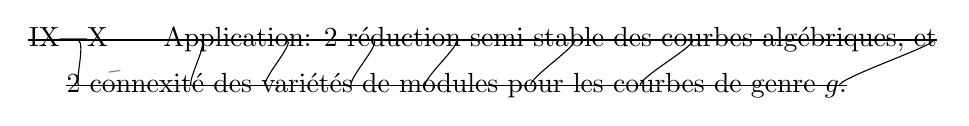
\begin{tikzpicture}
\node[anchor=west,inner sep=0pt] (a) at (0,0) {\deleted{\unsure{IX|X}}\qquad \deleted{Application: {\deleted{\illegible{2}}} réduction semi-stable des courbes algébriques, {\deleted{\unsure{et}}}}};
\node[anchor=west,inner sep=0pt] (b) at (.48,-.58) {\deleted{{\deleted{\illegible{2}}} \tikz[overlay]{\draw[gray] (.24,.26)--(.39,.28);}connexité des variétés de modules pour les courbes de genre $g$.}};
\draw (a.west) -- (a.east);
\draw (b.west) -- (b.east);
\foreach \p/\q in {.055/.016,.19/.16,.285/.255,.38/.365,.47/.46,.60/.595,.73/.735,.995/.99}
{\path (a.west) -- (a.east) coordinate[pos=\p] (t);
 \path (b.west) -- (b.east) coordinate[pos=\q] (u);
 \draw (t) .. controls +(0.09,-.05) and +(-.04,.09) .. (u);}
\end{tikzpicture}}}

% archive sheet number: 1
\par\clearpage
\normalmarginpar
\scanpage{3}
\noindent\hfill\margin{\unsure{zurück} \unsure{an|au} \unsure{·}\tikz[baseline=(g.base)]{\node[inner sep=0pt] (g) {G};\draw ([xshift=-1pt,yshift=-4pt]g.south west)--([xshift=4pt,yshift=1pt]g.south east);}}\par

\noindent SGA 7

\noindent D\quad $\underline{\overline{\mathrm{X}}}$\quad \unsure{Intersections|Intersection} \tikz[baseline]{\draw[line cap=round] (0,.035)--(.065,.04) (.12,.04)--(.151,.043) (.211,.034)--(.295,.057);}

\noindent D\quad $\underline{\overline{\mathrm{XI}}}$\quad Int. \unsure{complètes|completes}

\noindent D\quad $\underline{\overline{\mathrm{XII}}}$\quad \unsure{Quadriques|Quadrique}

\noindent D\quad $\underline{\overline{\mathrm{XIII}}}$\quad Points \unsure{quadr.} \unsure{ordinaires}. Pic-\unsure{Lef|lef} faible

\noindent D\quad $\underline{\overline{\mathrm{XIV}}}$\quad Formule \unsure{Milnor}

\diagram{\(\begin{array}{@{}ll@{}}
\text{D}&\underline{\overline{\mathrm{XV}}}\\
\text{D}&\underline{\overline{\mathrm{XVI}}}
\end{array}
\left\{\begin{array}{l}
\text{Picard\unsure{'}-Lefschetz}\\
\text{Picard-Lefschetz}
\end{array}\right.
\;\tikz[baseline]{\draw[gray,thin] (0,.86) .. controls (.035,.62) and (-.045,.06) .. (.013,-.23);}
\)}

\noindent K\quad
$\begin{array}{@{}c@{}}
\underline{\overline{\mathrm{XVII}}}\\[-2pt]
\underline{\overline{\mathrm{XVIII}}}
\end{array}\,\Bigg|$\quad
\unsure{Pinceaux} de Lefschetz~: \uline{existence} \tikz[baseline]{\draw[gray,thin] (.18,.62) .. controls (.19,.36) and (.08,.18) .. (.07,-.09) -- (.11,-.17);\draw[gray,thin] (.20,.58) .. controls (.15,.25) and (.01,-.02) .. (-.01,-.20) -- (-.035,-.16);\draw[line cap=round] (-.06,0)--(.17,.34) (-.04,-.015)--(.18,.31) (.03,.013)--(.25,.35);} \uline{\unsure{étude|études} \unsure{cohomologique|cohomologiques}}

\diagram{D\quad $\underline{\overline{\deleted{\unsure{\mathrm{XVIII}}}\mathrm{XIX}}}$\quad
\uuline{Th de Noether}
$\left\{\begin{array}{l}
\text{via \unsure{Hodge}-Deligne}\\
\text{via \uuline{\underline{\text{Katz}}}}
\end{array}\right.$}

\diagram{\begin{tabular}{@{}c@{\ }p{.84\linewidth}@{}}
$\mathrm{K}\left\{\rule{0pt}{12ex}\right.$ &
\begin{minipage}[c]{\linewidth}
\noindent $\deleted{\underline{\overline{\unsure{\mathrm{XIX}|\mathrm{XX}}}}}\;
\underline{\overline{\mathrm{XX}}}\deleted{\unsure{\mathrm{I}}}$\quad \unsure{Th.|Thr.} de Griffiths.

\noindent $\underline{\overline{\mathrm{XXI}}}$\quad \deleted{\unsure{Théorème|Théor}} Niveau de la coh. des \unsure{intersections} \unsure{complètes|completes}

\noindent $\underline{\overline{\mathrm{XXII}}}$\quad \deleted{\unsure{Form.|Fon.}} Calcul de la \unsure{fonction} $\deleted{\unsure{z}}\zeta$ mod $p$.
\end{minipage}
\end{tabular}}

\figure{\begin{tikzpicture}\draw (0,0) .. controls (.29\linewidth,.45) and (.76\linewidth,.57) .. (.98\linewidth,.46);\end{tikzpicture}}

\noindent Exposés \unsure{transcendants} (Lê Dũng Tráng ?)

\[
\underline{\mathbb{F}_{q}\qquad \#\qquad \mathrm{card}}\quad\unsure{.}
\]

% archive sheet number: 2
\par\clearpage
\normalmarginpar
\scanpage{4}
\noindent\margin{\vspace*{5.3\baselineskip}SGA 7}\par

% The two long pen strokes, including their returns at the bottom, cross several rows.
\begingroup
\small
\setlength{\arraycolsep}{3pt}
\renewcommand{\arraystretch}{2.05}
\diagram{\figure{\resizebox{\linewidth}{!}{%
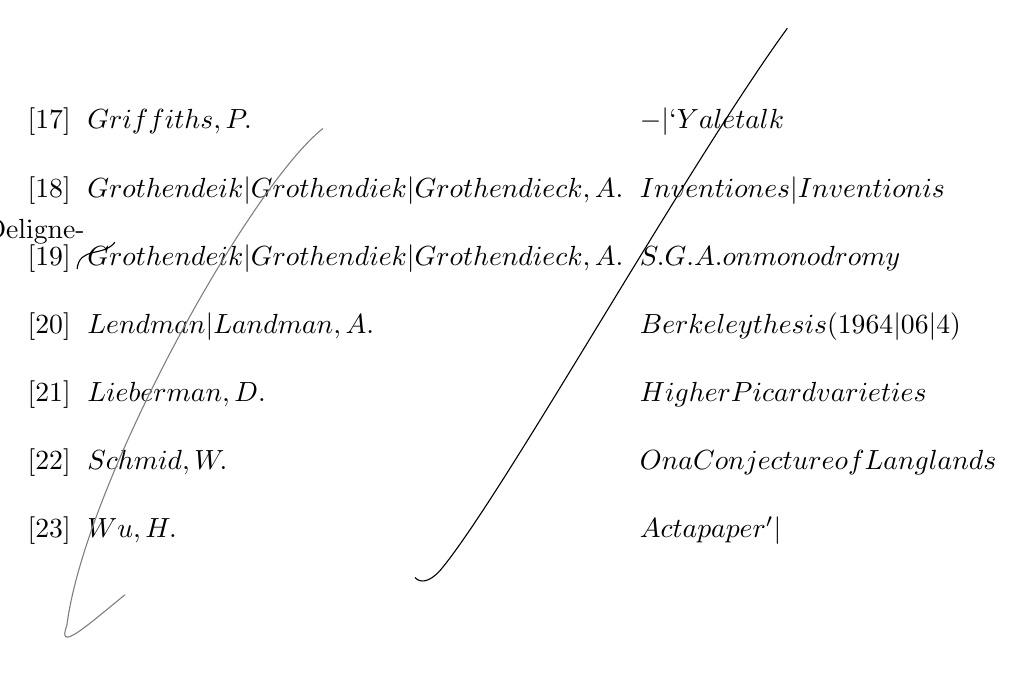
\begin{tikzpicture}
\node[anchor=south west,inner sep=0pt] (refs) at (0,0) {%
$\begin{array}{@{}lll@{}}
\text{[17]}&\text{Griffiths, P.}&\text{\unsure{-|\textquoteleft}Yale talk}\\
\text{[18]}&\text{\unsure{Grothendeik|Grothendiek|Grothendieck}, A.}&\text{\unsure{Inventiones|Inventionis}}\\
\text{[19]}&\text{\llap{\raisebox{.98em}{\inserted{Deligne-}\kern.1em}}\tikz[baseline,overlay]{\draw (-.13,-.05) .. controls (-.10,.24) and (.20,.10) .. (.35,.29);}\unsure{Grothendeik|Grothendiek|Grothendieck}, A.}&\text{S.G.A. on monodromy}\\
\text{[20]}&\text{\unsure{Lendman|Landman}, A.}&\text{Berkeley thesis (196\deleted{\unsure{4|0}}\unsure{6|4})}\\
\text{[21]}&\text{Lieberman, D.}&\text{Higher Picard varieties}\\
\text{[22]}&\text{Schmid, W.}&\text{On a Conjecture of Langlands}\\
\text{[23]}&\text{Wu, H.}&\text{Acta paper\unsure{\textquoteright|´}}
\end{array}$};
\begin{scope}[x={(refs.south east)},y={(refs.north west)}]
\draw[gray] (.305,.90) .. controls (.23,.78) and (.06,.16) .. (.041,-.14)
    .. controls (.030,-.20) and (.062,-.14) .. (.101,-.076);
\draw (.784,1.11) .. controls (.68,.82) and (.49,.13) .. (.426,-.025)
    .. controls (.414,-.052) and (.405,-.051) .. (.400,-.040);
\end{scope}
\end{tikzpicture}}}}
\endgroup

% archive sheet number: 3
\par\clearpage
\normalmarginpar
\scanpage{5}
\mspage{\handwritten{\tikz[baseline=(f.base)]{\node[inner sep=1pt] (f) {11bis};\draw (f.north west) .. controls ([yshift=-5pt]f.south west) and ([yshift=-5pt]f.south) .. ([yshift=-5pt]f.south east);}}}
\noindent\handwritten{\tikz[overlay]{\draw (-1.3,.30)--(-1.24,.41);\draw (-1.14,.41)--(-.99,.29);}}
\handwritten{\tikz[overlay]{\draw (.72\linewidth,.35) .. controls (.73\linewidth,.23) and (.732\linewidth,.23) .. (.733\linewidth,.35);}}
% The three large cancellation strokes cross the two numbered sections.
\figure{\begin{tikzpicture}
\node[anchor=north west,inner sep=0pt] (body) at (0,0) {\begin{minipage}{.93\linewidth}
\small
\noindent
\deleted{1.3.{\deleted{\unsure{2|3}}}{\unsure{3|2}}.}\quad
\deleted{\inserted{La terminologie de 1.3.1 {\deleted{et 1.3.2}} s'étend aussitôt au cas où}}
\deleted{\deleted{Revenons au cas {\unsure{où|ou}} on se donne deux Groupes $P$ et $Q$ sur $\unsure{G|S}$}}
\deleted{on a un {\uline{bitorseur}} {\deleted{\unsure{osus|sous}}} {\inserted{$E$}} sous{\deleted{\unsure{$(G$}}} $(G_{P},G_{P})$, {\deleted{resp{\unsure{.|,}} sous $(G_{P\mathrm{x}Q},G_{P\mathrm{x}Q})$,}} étant entendu qu'une rigidification du bitorseur $E$ doit être un isomorphisme de $e_{P}(E)$ avec le b{\deleted{\unsure{o}}}it{\deleted{\unsure{r|o}}}o{\deleted{\unsure{o|r}}}rs{\deleted{\unsure{e|u}}}eur trivial $\,{}_{s}G_{d}$, {\deleted{\unsure{donc}}} {\inserted{i.e.}}{\handwritten{\tikz[baseline]{\draw (0,-.04) .. controls (.035,.14) and (.16,.06) .. (.19,.25);}}} est défini par une section $e_{E}$ de $e_{P}(E)$ qui est {\uline{centrale}}, i.e. qui satisfait à la condition $g.e_{E}=e_{E}.g\quad(g\mathrel{\handwritten{\unsure{\in|\epsilon}}}G(S)$ . On étend de même la terminologie des birigidifications au cas des bitorseurs.}

\noindent\deleted{1.3.4.}\quad
\deleted{Revenons au cas où on se donne deux Groupes $P$ et {\deleted{$\handwritten{Q}$}} {\handwritten{\inserted{$G$}}}, et choisissons la section unité $e_{P}$ pour définir des rigidifications de bitorseurs sur $P$, et des birigidifications de bitorseurs sur $P\mathrm{x}P$. On a des foncteurs naturels}

\begingroup
\csname tagsleft@true\endcsname
\diagram{\[
\begin{tikzcd}[ampersand replacement=\&,column sep=1.7em]
\deleted{\underline{\mathrm{Ext}}(P;G)} \arrow[r,"{\handwritten{i}}"]
\& \deleted{\underline{\mathrm{Bitorsrig}}(P,G)} \arrow[r,"{\handwritten{\rlap{\raisebox{.35ex}{\hspace{-.12em}\(\color{gray!55}\scriptstyle\delta\)}}\delta}}"]
\& \deleted{\underline{\mathrm{Bitorsbirig}}(P,P;G){,}}
\end{tikzcd}
\tag*{\deleted{(1.3.4.1)}}
\]}
\endgroup

\noindent\deleted{où les trois expressions écrites désignent respectivement la catégorie des extensions de {\handwritten{\inserted{Groupes de}}} $P$ par $G$, la catégorie des {\deleted{b}}{\handwritten{B}}itorseurs sous $(G_{P},G_{P})$ rigidifiés pour{\unsure{\textasciigrave|\textquoteright}} $e_{P}$, et la catégorie des {\deleted{\unsure{t|b}}}b{\deleted{\unsure{o}}}it{\deleted{\unsure{r|o}}}orseurs sous$(G_{P\mathrm{x}P},G_{P\mathrm{x}P})$ birigidifiés pour $(e_{P},e_{P})$. On {\deleted{\unsure{prend}}} définit le foncteur $i$ en associant à l'extension $E$ de $P$ par $G$ le {\deleted{\unsure{torseu}}} bitorseur correspondant sur $P$ (1.1.6), rigidifié par la sectio{\unsure{ń|n}} unité de $E$. O{\deleted{\unsure{n}}}{\handwritten{n}} {\unsure{definit|définit}} le foncteur $\handwritten{\delta}$ par la formu{\deleted{\unsure{o|b}}}le}
\end{minipage}};
\begin{scope}[x={(body.north east)},y={(body.south west)}]
\draw (.44,.11) .. controls (.35,.27) and (.00,.66) .. (-.047,.725)
 .. controls (-.053,.736) and (-.054,.746) .. (-.043,.75);
\draw (.82,.078) .. controls (.73,.30) and (.50,.69) .. (.31,1.035);
\draw (.91,.505) .. controls (.915,.62) and (.78,.86) .. (.655,1.03);
\end{scope}
\end{tikzpicture}}
% archive sheet number: 4
